\chapter{Kết quả và Phân tích}
\label{ch:ketqua}

Toàn bộ log đầy đủ nằm trong \code{results/payment\_gateway\_v0/} và
\code{results/payment\_gateway\_v1/} nộp kèm (Phụ lục~\ref{app:logs}); chương này chỉ trích các
dòng quan trọng nhất. Môi trường: macOS 26 (arm64), Python 3.11.15, z3-solver 4.16.0, Apple clang
17.0.0, seed $=1$, ngân sách fuzzing 2\,000. Toàn bộ pipeline chạy trong khoảng 6 giây, trong đó
5,5 giây là biên dịch và chạy sanitizer.

% ============================================================
\section{Kết quả Chương 1 — Kripke và CTL}

\begin{figure}[H]
  \centering
  \adjustbox{max width=\linewidth, max height=0.55\textheight}{% Kripke: payment\_gateway\_v0 (sinh tự động bởi core.reporter)
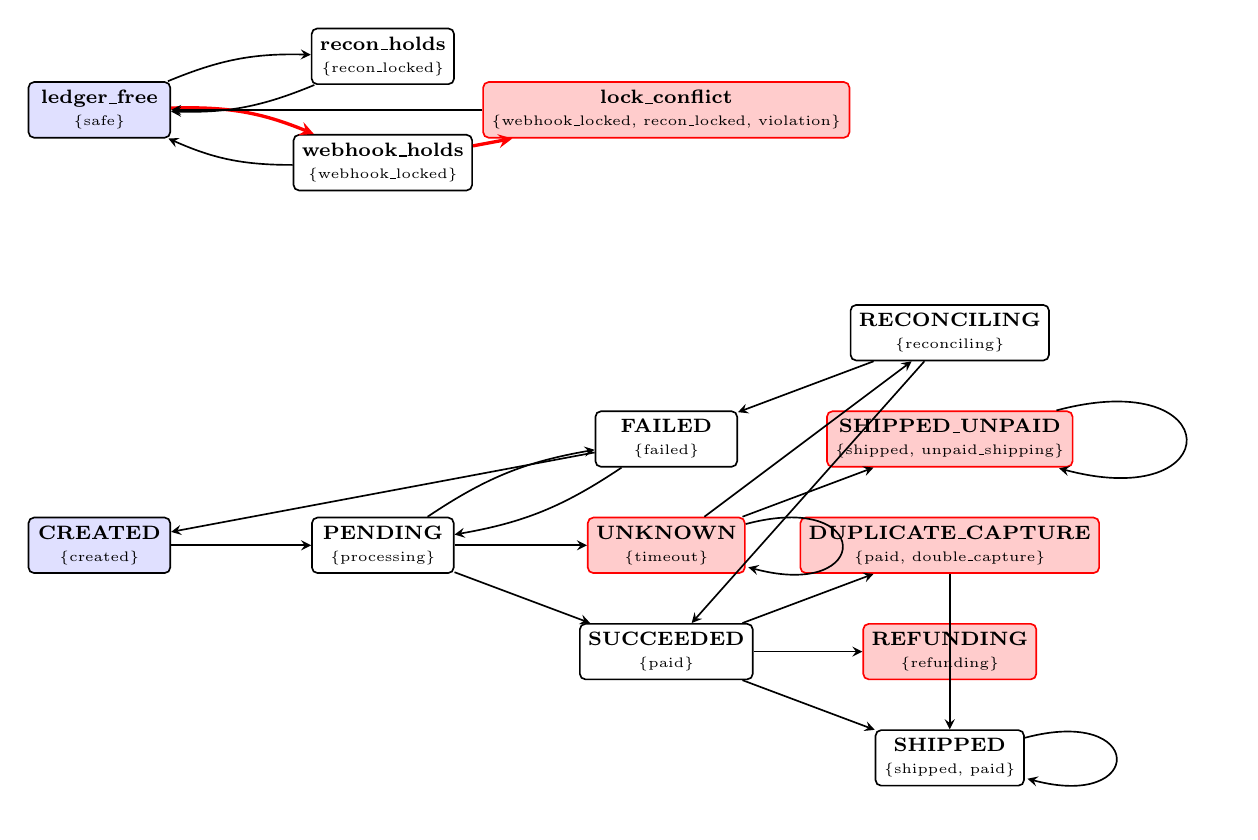
\begin{tikzpicture}[->,>=stealth,semithick,every node/.style={draw,rounded corners=2pt,align=center,font=\scriptsize,inner sep=3pt,minimum width=18mm}]
  \node[fill=blue!12] (n_ledger_free) at (0.00,-0.68) {\textbf{ledger\_free}\\{\tiny \{safe\}}};
  \node[fill=white] (n_webhook_holds) at (3.60,-1.35) {\textbf{webhook\_holds}\\{\tiny \{webhook\_locked\}}};
  \node[fill=white] (n_recon_holds) at (3.60,-0.00) {\textbf{recon\_holds}\\{\tiny \{recon\_locked\}}};
  \node[fill=red!20,draw=red] (n_lock_conflict) at (7.20,-0.68) {\textbf{lock\_conflict}\\{\tiny \{webhook\_locked, recon\_locked, violation\}}};
  \node[fill=blue!12] (n_CREATED) at (0.00,-6.21) {\textbf{CREATED}\\{\tiny \{created\}}};
  \node[fill=white] (n_PENDING) at (3.60,-6.21) {\textbf{PENDING}\\{\tiny \{processing\}}};
  \node[fill=red!20,draw=red] (n_UNKNOWN) at (7.20,-6.21) {\textbf{UNKNOWN}\\{\tiny \{timeout\}}};
  \node[fill=white] (n_RECONCILING) at (10.80,-3.51) {\textbf{RECONCILING}\\{\tiny \{reconciling\}}};
  \node[fill=white] (n_SUCCEEDED) at (7.20,-7.56) {\textbf{SUCCEEDED}\\{\tiny \{paid\}}};
  \node[fill=red!20,draw=red] (n_DUPLICATE_CAPTURE) at (10.80,-6.21) {\textbf{DUPLICATE\_CAPTURE}\\{\tiny \{paid, double\_capture\}}};
  \node[fill=white] (n_FAILED) at (7.20,-4.86) {\textbf{FAILED}\\{\tiny \{failed\}}};
  \node[fill=white] (n_SHIPPED) at (10.80,-8.91) {\textbf{SHIPPED}\\{\tiny \{shipped, paid\}}};
  \node[fill=red!20,draw=red] (n_SHIPPED_UNPAID) at (10.80,-4.86) {\textbf{SHIPPED\_UNPAID}\\{\tiny \{shipped, unpaid\_shipping\}}};
  \node[fill=red!20,draw=red] (n_REFUNDING) at (10.80,-7.56) {\textbf{REFUNDING}\\{\tiny \{refunding\}}};
  \draw[red,very thick,bend left=12] (n_ledger_free) to (n_webhook_holds);
  \draw[bend left=12] (n_ledger_free) to (n_recon_holds);
  \draw[bend left=12] (n_webhook_holds) to (n_ledger_free);
  \draw[red,very thick] (n_webhook_holds) to (n_lock_conflict);
  \draw[bend left=12] (n_recon_holds) to (n_ledger_free);
  \draw[] (n_lock_conflict) to (n_ledger_free);
  \draw[] (n_CREATED) to (n_PENDING);
  \draw[] (n_PENDING) to (n_SUCCEEDED);
  \draw[bend left=12] (n_PENDING) to (n_FAILED);
  \draw[] (n_PENDING) to (n_UNKNOWN);
  \draw[] (n_UNKNOWN) edge[loop right] (n_UNKNOWN);
  \draw[] (n_UNKNOWN) to (n_RECONCILING);
  \draw[] (n_UNKNOWN) to (n_SHIPPED_UNPAID);
  \draw[] (n_RECONCILING) to (n_SUCCEEDED);
  \draw[] (n_RECONCILING) to (n_FAILED);
  \draw[] (n_SUCCEEDED) to (n_SHIPPED);
  \draw[] (n_SUCCEEDED) to (n_DUPLICATE_CAPTURE);
  \draw[] (n_SUCCEEDED) to (n_REFUNDING);
  \draw[] (n_DUPLICATE_CAPTURE) to (n_SHIPPED);
  \draw[bend left=12] (n_FAILED) to (n_PENDING);
  \draw[] (n_FAILED) to (n_CREATED);
  \draw[] (n_SHIPPED) edge[loop right] (n_SHIPPED);
  \draw[] (n_SHIPPED_UNPAID) edge[loop right] (n_SHIPPED_UNPAID);
\end{tikzpicture}
}
  \caption{Mô hình Kripke của đặc tả v0 (sinh tự động). Trạng thái đỏ là trạng thái vi phạm;
           cạnh đỏ là phản ví dụ đầu tiên ($\mathbf{AG}\,\neg\mathit{violation}$).}
  \label{fig:kripke}
\end{figure}

\begin{table}[H]
\centering\small
\caption{Kết quả kiểm chứng CTL trên đặc tả v0 và v1 (trích \code{comparison.md}).}
\label{tab:ctlresult}
\begin{tabularx}{\linewidth}{@{}l l X l@{}}
\toprule
Thuộc tính & v0 & Phản ví dụ (v0) & v1 \\
\midrule
Deadlock & \textcolor{bad}{VI PHẠM} & \code{REFUNDING} không có chuyển tiếp ra & ĐẠT \\
P1 $\mathbf{AG}\,\neg\mathit{violation}$ & \textcolor{bad}{VI PHẠM} & ledger\_free $\to$ webhook\_holds $\to$ lock\_conflict & ĐẠT \\
P2 $\mathit{safe} \rightarrow \mathbf{EF}\,\mathit{webhook\_locked}$ & ĐẠT & — & ĐẠT \\
P3 $\mathbf{AG}(\mathit{shipped}\rightarrow\mathit{paid})$ & \textcolor{bad}{VI PHẠM} & CREATED $\to$ PENDING $\to$ UNKNOWN $\to$ SHIPPED\_UNPAID & ĐẠT \\
P4 $\mathbf{AG}(\mathit{timeout}\rightarrow\mathbf{AF}(\mathit{paid}\vee\mathit{failed}))$ & \textcolor{bad}{VI PHẠM} & CREATED $\to$ PENDING $\to$ UNKNOWN $\to$ UNKNOWN (lặp) & ĐẠT \\
P5 $\mathbf{AG}\,\neg\mathit{double\_capture}$ & \textcolor{bad}{VI PHẠM} & CREATED $\to$ PENDING $\to$ SUCCEEDED $\to$ DUPLICATE\_CAPTURE & ĐẠT \\
P6 $\mathbf{AG}\,\neg(\mathit{processing}\wedge\mathit{paid})$ & ĐẠT & — & ĐẠT \\
P7 $\mathit{created}\rightarrow\mathbf{EF}\,\mathit{shipped}$ & ĐẠT & — & ĐẠT \\
P8 $\mathbf{AG}(\mathit{refunding}\rightarrow\mathbf{AF}\,\mathit{refunded})$ & \textcolor{bad}{VI PHẠM} & CREATED $\to$ PENDING $\to$ SUCCEEDED $\to$ REFUNDING (kẹt) & ĐẠT \\
Mutex \code{webhook\_locked}/\code{recon\_locked} & \textcolor{bad}{VI PHẠM} & ledger\_free $\to$ webhook\_holds $\to$ lock\_conflict & ĐẠT \\
4 cặp mutex còn lại & ĐẠT & — & ĐẠT \\
\bottomrule
\end{tabularx}
\end{table}

\paragraph{Phân tích.}
\begin{itemize}
  \item \textbf{P1 / mutex (CWE-667):} từ \code{webhook\_holds} có cạnh sang \code{lock\_conflict}
        — worker đối soát lấy khóa khi worker webhook chưa nhả. v1 xóa cạnh này.
  \item \textbf{P3 (CWE-693, lỗi nghiệp vụ CWE-840):} thiết kế v0 cho phép ``giao hàng lạc quan''
        khi cổng timeout (\code{UNKNOWN} $\to$ \code{SHIPPED\_UNPAID}): hàng đi khi tiền chưa về.
        v1 bắt buộc \code{UNKNOWN} $\to$ \code{RECONCILING}.
  \item \textbf{P4:} phản ví dụ là một \emph{lasso}: \code{UNKNOWN} tự lặp (thăm dò cổng mãi) nên
        tồn tại một đường vô hạn không bao giờ đạt \code{paid} hay \code{failed}. Đây là lỗi mà
        không test case hữu hạn nào chứng minh được, nhưng model checking chỉ ra trực tiếp.
  \item \textbf{P5:} khi cổng gửi lại webhook (NFR-4), v0 ghi nhận thu tiền lần hai. v1 bỏ
        chuyển tiếp này (idempotency theo event ID).
  \item \textbf{P8 + deadlock (CWE-833):} \code{REFUNDING} không có chuyển tiếp ra. Nhờ quy ước
        ``stutter'' (trạng thái cụt được coi như tự lặp khi đánh giá CTL), P8 sai với phản ví dụ
        kẹt tại \code{REFUNDING}, đồng thời deadlock được báo riêng. Công cụ còn cảnh báo nhãn
        \code{refunded} không tồn tại trong mô hình v0 — dấu hiệu thiết kế thiếu trạng thái kết thúc.
\end{itemize}

\subsection{Bounded Model Checking}
\begin{table}[H]
\centering\small
\caption{Kết quả BMC (trích \code{logs/bmc.txt}).}
\label{tab:bmc}
\begin{tabular}{@{}l l l l@{}}
\toprule
Thuộc tính & v0 & $k$ vi phạm & v1 \\
\midrule
$\mathbf{AG}\,\neg\mathit{violation}$ & UNSAFE & 2 & SAFE, đạt CT $=4$ \\
$\mathbf{AG}(\mathit{shipped}\rightarrow\mathit{paid})$ & UNSAFE & 3 & SAFE, đạt CT $=4$ \\
$\mathbf{AG}\,\neg\mathit{double\_capture}$ & UNSAFE & 3 & SAFE, đạt CT $=4$ \\
$\mathbf{AG}\,\neg(\mathit{webhook\_locked}\wedge\mathit{recon\_locked})$ & UNSAFE & 2 & SAFE, đạt CT $=4$ \\
4 thuộc tính an toàn còn lại & SAFE, đạt CT $=3$ & — & SAFE, đạt CT $=4$ \\
\bottomrule
\end{tabular}
\end{table}

\begin{lstlisting}[style=logstyle,caption={Truy vết BMC cho $\mathbf{AG}(\mathit{shipped}\rightarrow\mathit{paid})$ trên v0 (trích \code{logs/bmc.txt}).}]
BMC AG(shipped -> paid): UNSAFE
  k=0   BMC_k unsat
  k=1   BMC_k unsat
  k=2   BMC_k unsat
  k=3   BMC_k sat
  Counterexample:
    s_0 = CREATED
    s_1 = PENDING
    s_2 = UNKNOWN
    s_3 = SHIPPED_UNPAID
\end{lstlisting}
BMC cho cùng phản ví dụ với model checking nhưng thêm thông tin \emph{độ sâu tối thiểu}: không
có đường vi phạm nào ngắn hơn 3 bước. Với v1, $\mathit{BMC}_k$ UNSAT với mọi $k \le 4 = CT$, nên
kết luận an toàn là đầy đủ, không chỉ ``an toàn đến độ sâu $k$''.

% ============================================================
\section{Phân tích từng lỗ hổng và bản vá}
\label{sec:cwe}
Mỗi lỗ hổng được trình bày theo 5 mục: vị trí, nguyên nhân gốc rễ, bằng chứng tồn tại, cách vá,
bằng chứng đã vá. Mã trích từ \code{results/payment\_gateway\_v0/source/}.

% ------------------------------------------------------------
\subsection{\cwe{120}{Buffer Copy without Checking Size of Input} tại \code{parse\_webhook\_signature}}
\textbf{(1) Vị trí.} \code{parse\_webhook\_signature\_v0.c}, dòng 9; truy vết REQ-5, CON-1.

\textbf{(2) Nguyên nhân gốc rễ.} \code{strcpy} sao chép tới khi gặp \code{'\textbackslash 0'} mà
không biết kích thước bộ đệm đích (65 byte trên stack). Chữ ký do bên ngoài kiểm soát (vượt trust
boundary, Hình~\ref{fig:kientruc}), nên chuỗi dài hơn 64 ký tự ghi đè vùng stack kề cận, có thể
tới địa chỉ trả về (Chương 2.3).

\textbf{(3) Bằng chứng lỗi tồn tại.} Scanner: \code{dangerous-function} tại dòng 9. ASan với
input 520 ký tự:
\begin{lstlisting}[style=logstyle,caption={Trích \code{logs/sanitizer\_parse\_webhook\_signature\_v0.log}.}]
==46110==ERROR: AddressSanitizer: stack-buffer-overflow on address 0x00016bad2521
WRITE of size 521 at 0x00016bad2521 thread T0
    #1 in parse_webhook_signature parse_webhook_signature_v0.c:9
SUMMARY: AddressSanitizer: stack-buffer-overflow parse_webhook_signature_v0.c:9
\end{lstlisting}

\textbf{(4) Cách vá.}

\noindent\begin{minipage}[t]{0.49\linewidth}
\begin{lstlisting}[language=C,caption={v0 — có lỗi}]
int parse_webhook_signature(
    const char *raw_signature) {
  char buffer[65];
  strcpy(buffer, raw_signature);
  printf("%s\n", buffer);
  return 0;
}
\end{lstlisting}
\end{minipage}\hfill
\begin{minipage}[t]{0.49\linewidth}
\begin{lstlisting}[language=C,caption={v1 — đã vá}]
int parse_webhook_signature(
    const char *raw_signature) {
  char buffer[65];
  if (raw_signature == NULL) return -1;
  size_t len = strnlen(raw_signature,
                       sizeof buffer);
  if (len >= sizeof buffer) return -1;
  memcpy(buffer, raw_signature, len);
  buffer[len] = '\0';
  printf("%s\n", buffer);
  return 0;
}
\end{lstlisting}
\end{minipage}

Bản vá \emph{từ chối} chữ ký quá dài thay vì cắt bớt âm thầm như \code{strncpy}: một chữ ký bị cắt
có thể vẫn được so khớp một phần, còn từ chối loại bỏ hẳn nguyên nhân gốc. Cùng khuôn mẫu này được
dùng cho \code{parse\_order\_id}, hàm không có lỗi khai báo: scanner và ASan đều cho 0 finding trên
cả hai phiên bản (không báo nhầm).

\textbf{(5) Bằng chứng đã vá.} Scanner v1: 0 finding. ASan v1 với cùng input 520 ký tự: thoát mã 0,
không có báo cáo, hàm trả về \code{rc=-1} (từ chối).

% ------------------------------------------------------------
\subsection{\cwe{415}{Double Free} tại \code{close\_payment\_session}}
\textbf{(1) Vị trí.} \code{close\_payment\_session\_v0.c}, dòng 13; truy vết REQ-7.

\textbf{(2) Nguyên nhân gốc rễ.} Con trỏ \code{data} được \code{free} ở dòng 12 rồi lại ở dòng 13;
lần thứ hai làm hỏng metadata của heap allocator và có thể bị khai thác để ghi tùy ý
(Chương 2.2). Trong hệ thống thật, lỗi xuất hiện khi hai luồng cùng đóng một phiên.

\textbf{(3) Bằng chứng lỗi tồn tại.}
\begin{lstlisting}[style=logstyle,caption={Scanner và ASan trên v0.}]
close_payment_session_v0.c:13: [HIGH] double-free CWE-415: free('data') lan hai (da free() tai dong 12)
==46141==ERROR: AddressSanitizer: attempting double-free on 0x6020000000d0 in thread T0:
    #1 in close_payment_session close_payment_session_v0.c:13
freed by thread T0 here:
    #1 in close_payment_session close_payment_session_v0.c:12
previously allocated by thread T0 here:
    #1 in close_payment_session close_payment_session_v0.c:8
\end{lstlisting}
Hai công cụ độc lập (tĩnh và động) chỉ ra cùng dòng 12/13.

\textbf{(4) Cách vá.}

\noindent\begin{minipage}[t]{0.49\linewidth}
\begin{lstlisting}[language=C,caption={v0 — có lỗi}]
data[0] = 'A';
free(data);
free(data);
return 0;
\end{lstlisting}
\end{minipage}\hfill
\begin{minipage}[t]{0.49\linewidth}
\begin{lstlisting}[language=C,caption={v1 — đã vá}]
data[0] = 'A';
free(data);
data = NULL;  /* free(NULL) vo hai */
return 0;
\end{lstlisting}
\end{minipage}

\textbf{(5) Bằng chứng đã vá.} Scanner v1: 0 finding; ASan v1: sạch.

% ------------------------------------------------------------
\subsection{\cwe{416}{Use After Free} và \cwe{401}{Memory Leak}}
\code{release\_card\_token\_buffer\_v0.c} dòng 12 ghi \code{data[0]} sau khi \code{free} ở dòng 11:
scanner báo \code{use-after-free}, ASan báo \code{heap-use-after-free} tại cùng dòng.
\code{write\_audit\_log\_v0.c} dòng 12 thoát hàm khi vùng nhớ cấp phát ở dòng 8 chưa được giải
phóng: scanner báo \code{memory-leak}. Bản v1 của cả hai hàm giải phóng đúng một lần rồi gán
\code{NULL}; scanner và ASan v1 đều sạch. Lưu ý: CWE-401 chỉ có bằng chứng tĩnh vì LeakSanitizer
không hỗ trợ macOS (xem Chương~\ref{ch:thaoluan}).

% ------------------------------------------------------------
\subsection{\cwe{190}{Integer Overflow or Wraparound}}
\textbf{(1) Vị trí.} \code{calculate\_total\_payment\_v0.c} dòng 5 (\code{*out = amount +
shipping\_fee}) và 6 bộ đếm trong sheet \code{KiemTraSoHoc}; truy vết REQ-9, CON-4.

\textbf{(2) Nguyên nhân gốc rễ.} Cộng hai \code{int} có dấu vượt $2^{31}-1$ là undefined behavior;
thực tế thường wrap-around thành số âm, khiến tổng tiền cần thu âm hoặc rất nhỏ — lỗi số học dẫn
thẳng tới lỗi nghiệp vụ (CWE-840).

\textbf{(3) Bằng chứng.} UBSan trên v0 với \code{(INT\_MAX, 1)}:
\begin{lstlisting}[style=logstyle,caption={Trích \code{logs/sanitizer\_calculate\_total\_payment\_v0.log}.}]
calculate_total_payment_v0.c:5:19: runtime error: signed integer overflow:
    2147483647 + 1 cannot be represented in type 'int'
\end{lstlisting}

\begin{table}[H]
\centering\small
\caption{Kết quả SMT (trích \code{logs/z3.txt}); mọi biến trong miền int32.}
\label{tab:smt}
\begin{tabularx}{\linewidth}{@{}l l X r l@{}}
\toprule
Kiểm tra & Ngưỡng & Model tràn (thỏa điều kiện nghiệp vụ) & Wrap 32-bit & Sau vá \\
\midrule
order\_total\_counter & int32 & amount $=2\,147\,483\,647$, shipping\_fee $=1$ & $-2\,147\,204\,848$ & UNSAT \\
daily\_transaction\_counter & int16 & tx\_today $=2\,147\,483\,647$, tx\_backlog $=1$ & $-2\,129\,640\,465$ & UNSAT \\
active\_session\_counter & uint16 & active $=2\,147\,483\,647$, pending $=1$ & $-2\,145\,843\,031$ & UNSAT \\
refund\_total\_vnd & int32 & refunded $=2\,147\,483\,647$, pending $=1$ & $-2\,143\,285\,231$ & UNSAT \\
webhook\_retry\_counter & int16 & today $=2\,147\,483\,647$, backlog $=1$ & $-2\,111\,565\,480$ & UNSAT \\
settlement\_batch\_bytes & int32 & batch $=2\,147\,483\,647$, header $=1$ & $-2\,145\,771\,516$ & UNSAT \\
\bottomrule
\end{tabularx}
\end{table}
Cột ``Wrap 32-bit'' là kết quả mà một \code{int} của C thực sự tính ra (lý thuyết bit-vector). Ví
dụ với \code{order\_total\_counter}, Z3 tìm được
$1\,073\,758\,211 + 1\,074\,004\,237 = -2\,147\,204\,848$: hai khoản tiền dương cho tổng âm.

\textbf{(4) Cách vá.} Kiểm tra \code{(b > 0 \&\& a > INT\_MAX - b) || (b < 0 \&\& a < INT\_MIN - b)}
trước khi cộng và trả lỗi (\code{calculate\_total\_payment\_v1.c}).

\textbf{(5) Bằng chứng đã vá.} UBSan v1 sạch với cùng input. Với cả 6 bộ đếm, truy vấn tràn số
kèm tiền điều kiện của bản vá trả về \textbf{UNSAT} — một \emph{chứng minh toán học} rằng không
tồn tại input int32 nào gây tràn, mạnh hơn mọi test case.

% ------------------------------------------------------------
\subsection{\cwe{369}{Divide By Zero} tại \code{refund\_ratio} và \cwe{798}{Hard-coded Credentials}}
Bằng chứng của hai lớp lỗi này đến từ fuzzing (Mục~\ref{sec:fuzz}). \code{refund\_ratio} v0 chia
\code{refund\_amount // total\_amount} không kiểm tra mẫu số; v1 trả 0 khi mẫu số bằng 0.
\code{webhook\_bypass\_token} và \code{support\_override\_pin} v0 trả \code{True} khi hai tham số
bằng cặp hằng số (7788, 9999) và (4821, 7306) — cửa hậu hardcode. v1 so khớp với bí mật cấu hình
ngoài mã nguồn bằng \code{hmac.compare\_digest} (so sánh thời gian hằng) và từ chối khi chưa cấu
hình.

% ============================================================
\section{So sánh các chiến lược fuzzing}
\label{sec:fuzz}
\begin{table}[H]
\centering\small
\caption{Fuzzing với ngân sách 2\,000 lần thử, seed $=1$ (trích \code{logs/fuzz.csv}).}
\label{tab:fuzz}
\footnotesize
\begin{tabular}{@{}l l r r l l@{}}
\toprule
Hàm (v0) & Chiến lược & Lần thử chạy & Số lần lỗi & Lần đầu & Input gây lỗi \\
\midrule
\code{refund\_ratio} & Black-box & 2000 & 47 & 48 & (2147483646, 0) \\
\code{refund\_ratio} & Coverage-guided & 2000 & 24 & 6 & (1, 0) \\
\code{refund\_ratio} & Concolic & 3 & 1 & 2 & ($-2147483648$, 0) \\
\code{webhook\_bypass\_token} & Black-box & 2000 & 0 & — & — \\
\code{webhook\_bypass\_token} & Coverage-guided & 2000 & 0 & — & — \\
\code{webhook\_bypass\_token} & Concolic & 5 & 1 & 4 & (7788, 9999) \\
\code{support\_override\_pin} & Black-box & 2000 & 0 & — & — \\
\code{support\_override\_pin} & Coverage-guided & 2000 & 0 & — & — \\
\code{support\_override\_pin} & Concolic & 5 & 1 & 4 & (4821, 7306) \\
\midrule
Cả 3 hàm, bản v1 & Cả 3 chiến lược & 2000 & 0 & — & — \\
\bottomrule
\end{tabular}
\end{table}

\paragraph{Phân tích.}
\begin{itemize}
  \item \code{refund\_ratio} là lỗi ``nông'': mọi chiến lược đều tìm ra. Black-box tìm được nhờ
        30\% input lấy từ tập giá trị biên có chứa 0 — không có tập này, xác suất trúng
        \code{total\_amount = 0} ngẫu nhiên chỉ là $2^{-32}$ mỗi lần.
  \item Với mã bí mật, xác suất một cặp int32 ngẫu nhiên trúng đúng cặp là $2^{-64}$: black-box
        thất bại hoàn toàn sau 2\,000 lần, đúng như Chương 4.5.
  \item Coverage-guided \emph{cũng} thất bại: điều kiện \code{header\_token == 7788} không mở
        dòng mã mới cho tới khi khớp chính xác, nên tín hiệu coverage không tăng dần — đây là
        ``vấn đề magic byte'' (Chương 4.3--4.6) mà AFL giải bằng CmpLog/laf-intel.
  \item Concolic thu path condition $\mathit{header\_token} = 7788 \wedge \mathit{secret\_token}
        = 9999$ từ AST rồi giải trực tiếp bằng Z3, tìm ra cửa hậu ở lần chạy thứ 4 và dừng khi
        hết nhánh để phủ định (chỉ 5 lần chạy).
  \item Trên v1, concolic dừng sau 1 lần chạy vì hàm gọi \code{os.environ}/\code{hmac} mà engine
        không mô hình hóa được — giới hạn ``environment modeling'' của symbolic execution
        (Chương 4.6), được ghi nhận trong \code{logs/fuzz\_events.txt}.
\end{itemize}

% ============================================================
\section{Bảng tổng hợp trước/sau}
\begin{table}[H]
\centering\small
\caption{Tổng hợp lỗ hổng và trạng thái trước/sau (rút gọn từ \code{before\_after.md} và \code{comparison.md}).}
\label{tab:beforeafter}
\footnotesize
\begin{tabularx}{\linewidth}{@{}l >{\raggedright\arraybackslash}p{3.1cm} >{\raggedright\arraybackslash}X >{\raggedright\arraybackslash}X >{\raggedright\arraybackslash}p{1.9cm}@{}}
\toprule
CWE & Vị trí & Trạng thái v0 & Trạng thái v1 & Công cụ xác minh \\
\midrule
CWE-120 & \code{parse\_webhook\_signature} & ASan stack-buffer-overflow dòng 9 (WRITE 521 byte) & Từ chối input $>64$ ký tự; 0 finding, ASan sạch & Scanner + ASan \\
CWE-401 & \code{write\_audit\_log} & Scanner: không free trước return, dòng 12 & 0 finding & Scanner \\
CWE-415 & \code{close\_payment\_session} & ASan attempting double-free dòng 13 & 0 finding, ASan sạch & Scanner + ASan \\
CWE-416 & \code{release\_card\_token\_buffer} & ASan heap-use-after-free dòng 12 & 0 finding, ASan sạch & Scanner + ASan \\
CWE-190 & \code{calculate\_total\_payment} & UBSan signed overflow dòng 5 & UBSan sạch & UBSan \\
CWE-190 & 6 bộ đếm & Z3 SAT, wrap thành số âm & Z3 UNSAT với tiền điều kiện & Z3 \\
CWE-369 & \code{refund\_ratio} & ZeroDivisionError, 47/2000 lần (black-box) & 0/2000 cả 3 chiến lược & Fuzzing \\
CWE-798 & \code{webhook\_bypass\_token} & Bypass với (7788, 9999), concolic lần 4 & 0/2000 & Concolic \\
CWE-798 & \code{support\_override\_pin} & Bypass với (4821, 7306), concolic lần 4 & 0/2000 & Concolic \\
CWE-667 & Khóa sổ cái & Mutex vi phạm, phản ví dụ độ dài 2 & ĐẠT; BMC SAFE đạt CT & CTL + BMC \\
CWE-693 & P3, P4, P5, P8 & 4 thuộc tính CTL sai, có phản ví dụ & Cả 4 ĐẠT & CTL + BMC \\
CWE-833 & \code{REFUNDING} & Deadlock & Không deadlock & Kripke \\
\bottomrule
\end{tabularx}
\end{table}

% ============================================================
\section{Truy vết test case}
\begin{table}[H]
\centering\small
\caption{Test case truy vết từ đặc tả, đánh giá tự động (trích \code{comparison.md}).}
\label{tab:tc}
\begin{tabularx}{\linewidth}{@{}l l X l l@{}}
\toprule
ID & Yêu cầu & Kết quả mong đợi & v0 & v1 \\
\midrule
TC-1 & REQ-3, REQ-4 & AG(!violation) ĐÚNG và không có trạng thái deadlock & FAIL & PASS \\
TC-2 & REQ-1 & AG(shipped -> paid) ĐÚNG & FAIL & PASS \\
TC-3 & REQ-2 & AG(timeout -> AF(paid | failed)) ĐÚNG & FAIL & PASS \\
TC-4 & REQ-12, NFR-4 & AG(!double\_capture) ĐÚNG & FAIL & PASS \\
TC-5 & REQ-13 & AG(refunding -> AF(refunded)) ĐÚNG và không có deadlock & FAIL & PASS \\
TC-6 & REQ-5, CON-1 & Không phát hiện CWE-120 tại parse\_webhook\_signature & FAIL & PASS \\
TC-7 & REQ-6, 7, 8 & Không phát hiện CWE-401, CWE-415, CWE-416 & FAIL & PASS \\
TC-8 & REQ-9, CON-4 & Không phát hiện CWE-190 tại calculate\_total\_payment & FAIL & PASS \\
TC-9 & REQ-9 & Z3 SAT khi chưa kiểm tra biên và UNSAT sau khi thêm tiền điều kiện & PASS & PASS \\
TC-10 & REQ-10 & Không crash (ZeroDivisionError) tại refund\_ratio & FAIL & PASS \\
TC-11 & REQ-11, CON-6 & Không phát hiện CWE-798 & FAIL & PASS \\
TC-12 & REQ-14, CON-2 & Không phát hiện CWE-120 tại parse\_order\_id & PASS & PASS \\
\midrule
\multicolumn{3}{@{}l}{Tổng} & 2/12 & 12/12 \\
\bottomrule
\end{tabularx}
\end{table}
TC-12 PASS trên cả hai phiên bản là kiểm tra \emph{âm tính}: hàm không có lỗi khai báo thì công cụ
không được báo nhầm. TC-9 PASS trên v0 vì nó kiểm tra chính khả năng chứng minh của Z3, không kiểm
tra mã v0.
